%%
%% Copyright 2007, 2008, 2009 Elsevier Ltd
%%
%% This file is part of the 'Elsarticle Bundle'.
%% ---------------------------------------------
%%
%% It may be distributed under the conditions of the LaTeX Project Public
%% License, either version 1.2 of this license or (at your option) any
%% later version.  The latest version of this license is in
%%    http://www.latex-project.org/lppl.txt
%% and version 1.2 or later is part of all distributions of LaTeX
%% version 1999/12/01 or later.
%%
%% The list of all files belonging to the 'Elsarticle Bundle' is
%% given in the file `manifest.txt'.
%%

%% Template article for Elsevier's document class `elsarticle'
%% with numbered style bibliographic references
%% SP 2008/03/01
%%
%%
%%
%% $Id: elsarticle-template-num.tex 4 2009-10-24 08:22:58Z rishi $
%%
%%
\documentclass[preprint,12pt,3p]{elsarticle}

%% Use the option review to obtain double line spacing
%% \documentclass[preprint,review,12pt]{elsarticle}

%% Use the options 1p,twocolumn; 3p; 3p,twocolumn; 5p; or 5p,twocolumn
%% for a journal layout:
%% \documentclass[final,1p,times]{elsarticle}
%% \documentclass[final,1p,times,twocolumn]{elsarticle}
%% \documentclass[final,3p,times]{elsarticle}
%% \documentclass[final,3p,times,twocolumn]{elsarticle}
%% \documentclass[final,5p,times]{elsarticle}
%% \documentclass[final,5p,times,twocolumn]{elsarticle}

%% if you use PostScript figures in your article
%% use the graphics package for simple commands
%% \usepackage{graphics}
%% or use the graphicx package for more complicated commands
%% \usepackage{graphicx}
%% or use the epsfig package if you prefer to use the old commands
%% \usepackage{epsfig}


\usepackage{amssymb}
\usepackage{amsthm}
\usepackage{amsmath}
\usepackage{mathrsfs}
\usepackage{algorithm}
\usepackage{algorithmic}
\usepackage{graphicx}
\usepackage{grffile}

%% The lineno packages adds line numbers. Start line numbering with
%% \begin{linenumbers}, end it with \end{linenumbers}. Or switch it on
%% for the whole article with \linenumbers after \end{frontmatter}.
%% \usepackage{lineno}

%% natbib.sty is loaded by default. However, natbib options can be
%% provided with \biboptions{...} command. Following options are
%% valid:

%%   round  -  round parentheses are used (default)
%%   square -  square brackets are used   [option]
%%   curly  -  curly braces are used      {option}
%%   angle  -  angle brackets are used    <option>
%%   semicolon  -  multiple citations separated by semi-colon
%%   colon  - same as semicolon, an earlier confusion
%%   comma  -  separated by comma
%%   numbers-  selects numerical citations
%%   super  -  numerical citations as superscripts
%%   sort   -  sorts multiple citations according to order in ref. list
%%   sort&compress   -  like sort, but also compresses numerical citations
%%   compress - compresses without sorting
%%
%% \biboptions{comma,round}

% \biboptions{}
\newcommand{\bx}{\mathbf{x}}
\newcommand{\R}{\mathbb{R}}
\newcommand{\D}{\mathscr{D}}
\newcommand{\N}{\mathscr{N}}
\newcommand{\by}{\mathbf{y}}
\DeclareMathOperator*{\argmin}{\arg\!\min}

\newtheorem{conjecture}{Conjecture}
\newtheorem{theorem}{Theorem}
\newtheorem{experiment}{Experiment}

\journal{STAT 241A}

\begin{document}

\begin{frontmatter}

\title{A Novel Sampling Method Using Stochastic Gradient Descent}


\author{Yu Wang, 3031741324\\ Weixin Cai, 26954913}
%\address[label2]{Address Two\fnref{label4}}

\begin{abstract}
Stochastic gradient descent (SGD), under mild conditions, can be viewed as a Markov chain. This relationship has been pointed out in a variety of papers \cite{kushner2012stochastic, bach2014adaptivity}. Although SGD has been extensively studied, its property as a Markov chain seems to be largely overlooked. What is its stationary distribution? What is its mixing time? How does its mixing time relate to its convergence rate? Studying these properties could offer a novel perspective to understand SGD.

Currently, there aren't a lot of schemes available to analyzing SGD's mixing time. Traditional ways includes coupling, diameter bounds, and bottle-neck ratio etc. (see \emph{Reversible Markov chains and random walks on graphs} by Aldous et al.\cite{aldous2002reversible}, and \emph{Markov chains and mixing times} by Levin et al.\cite{levin2009markov}). However, these methods are designed for the Markov chain on a graph and might not be able to be applied to SGD directly.

Our proposal is to bridge the gap between classical Markov chain analysis and SGD. Specifically,  we would like to explore mixing time related issues and obtain some novel theoretical and empirical findings on the mixing time of SGD (If successful). A specific question to answer is whether lower mixing time will imply faster convergence rate. The hunch is that if the corresponding Markov chain has a low mixing time, SGD should converge fast. This seems to be a novel perspective to understand SGD. Duchi et al.\cite{duchi2012ergodic} shows how the finite-sample convergence rate (expected convergence \& high-probability convergence) of stochastic sub-gradient descent depends on the mixing time of the process. If we can bound the mixing time, subsequently, we will be able to understand the convergence of this class of optimization techniques. Theoretical analysis as well as empirical experiments will be carried out to further explore this issue.

Our group contains two people. The tentative plan is that Yu focuses on the theoretical exploration and Weixin focuses on the empirical experiments. The final report will be written together.
\end{abstract}

\begin{keyword}
%% keywords here, in the form: keyword \sep keyword
Stochastic gradient descent \sep Sampling \sep Metropolis-Hastings
%% MSC codes here, in the form: \MSC code \sep code
%% or \MSC[2008] code \sep code (2000 is the default)
\end{keyword}

\end{frontmatter}

%%
%% Start line numbering here if you want
%%
% \linenumbers
% ===================================================================================
\section{Introduction} % (fold)
\label{sec:introduction}

% section introduction (end)


% ===================================================================================
%% main text
\section{Main Theorems}

\begin{algorithm}
{\small
Given objective function $h(x)$, stepsize $\alpha$, noise level $\sigma^2$,
\begin{algorithmic}\caption{Stochastic gradient descent}\label{Alg:SGD}
\STATE {\bf Initialize} $ \bx^0$ arbitrarily;
\WHILE{stopping criterion not satisfied}
\STATE draw $\epsilon^t$ from Gaussian distribution $\N(0, \sigma^2)$.
\STATE
$\bx^{k+1} \gets \bx^k - \alpha(\nabla f(\bx^k) + \epsilon^t)$;
\STATE $k\gets k+1$;
\ENDWHILE
\STATE return $\bx^k$.
\end{algorithmic}}
\end{algorithm}

Define $\D(\R^p)$ to be the family of the density functions of smooth random variables in $\R^p$, i.e.,

\begin{equation}
\D(\R^p)\triangleq \{p(\bx)\Big| p\in C^1(\R^p),~p(\bx) \geq 0,~ \int_\bx p(\bx) = 1.\}
\end{equation}
Consider any $p(\bx)\in \D(\R^p)$, we have the following theorem:

\begin{conjecture}
For any $p(\bx)\in \D(\R^p)$, it is the stationary distribution of iterates in Algorithm 1 with parameter $(-\log p(\bx), \epsilon, 2\epsilon)$.
\end{conjecture}
\begin{proof}
Let's verify this theorem by checking the detailed balance condition. Denote $g(\by|\bx)$ to be the density function of the transition, because $\by = \bx - \alpha \nabla f(\bx^k) + \epsilon^t$ and $\epsilon^t\sim \N(0, \sigma^2)$, we know
\begin{equation}
g(\by|\bx) = (2\pi \sigma^2)^{-p/2} \exp(- \frac{\|\by - \bx + \alpha \nabla h(\bx)\|^2}{2\sigma^2}).
\end{equation}
Then the detailed balance condition is
\begin{equation}\label{Eq:detailBalance}
p(\bx^{k+1}) g(\bx^{k}|\bx^{k+1}) = p(\bx^{k}) g(\bx^{k+1}|\bx^{k}).
\end{equation}
Since we will only consider $\bx^k$ and $\bx^{k+1}$ in the proof. For notation ease, we denote $\bx^{k+1}$ as $\bx^+$.
In order to prove \ref{Eq:detailBalance}, we would like to show the ratio between LHS and RHS to be 1. To be more specific, we have (Recall that $\sigma^2 = \alpha$)
\begin{eqnarray}
\frac{p(\bx^{+}) g(\bx^{k}|\bx^{+})}{p(\bx^{k}) g(\bx^{+}|\bx^{k})} = & \exp(-h(\bx^{+}) - \frac{\|\bx^{k} - \bx^+ + \alpha \nabla h(\bx^{+})\|^2}{2\alpha} + h(\bx^{k}) + \frac{\|\bx^{+} - \bx^k + \alpha \nabla h(\bx^k)\|^2}{2\alpha}).
\end{eqnarray}
Note that
\[h(\bx^+) - h(\bx^k) = \frac{\nabla h(\bx^k) + \nabla h(\bx^+)}{2} \cdot (\bx^+ - \bx^k) + O(\|\bx^+ - \bx^k\|^2),
\]
and
\begin{eqnarray}
 & \frac{\|\bx^{k} - \bx^+ + \alpha \nabla h(\bx^{+})\|^2}{2\alpha} - \frac{\|\bx^{+} - \bx^k + \alpha \nabla h(\bx^k)\|^2}{2\alpha} \\
 =& -\frac{\nabla h(\bx^k) + \nabla h(\bx^+)}{2} \cdot (\bx^+ - \bx^k) + \alpha/2 \|\nabla h(\bx^+)\|^2 - \alpha/2 \|\nabla h(\bx^+)\|^2.
\end{eqnarray}
Here, $\|\bx^+ - \bx^k\|$ will be roughly no bigger than $\alpha$ because $\bx^+ = \bx^k - \alpha \nabla h(\bx^k) + \epsilon^k$.  Thus it means $O(\|\bx^+ - \bx^k\|) = O(\alpha^2)$. What's more, $\alpha/2 \|\nabla h(\bx^+)\|^2 - \alpha/2 \|\nabla h(\bx^+)\|^2 = O(\alpha^2)$.
Thus we know
\begin{eqnarray}
\log \frac{p(\bx^{+}) g(\bx^{k}|\bx^{+})}{p(\bx^{k}) g(\bx^{+}|\bx^{k})} = &O(\alpha^2).
\end{eqnarray}
Therefore, we know the detailed balance equality holds approximately especially when $\alpha$ is small.

When $h$ is a quadratic function, the detailed balance holds exactly.
\end{proof}

Some empirical demonstration. How accurate is this approximation?

Since this is only a very rough deduction, we would like to examine the stationary distribution of SGD empirically for some special cases.

\begin{experiment}
Take the density function of $X$ to be $f(x) \propto \exp(- x^4)$, let $2\sigma^2 = \epsilon = 0.005$, $x_0 = 1$, burning-in period is $1000$, waiting period is $1000$, the empirical histogram v.s. the desired histogram is plotted in Figure ???
\end{experiment}
\begin{figure}
    \centering
    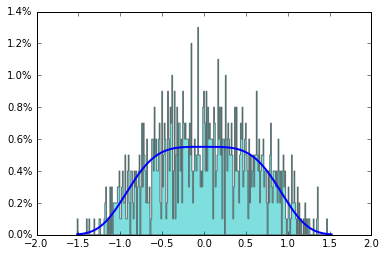
\includegraphics{../figure/case1_step_0.005_iter_1e3.png}
    \caption{Experiment 1: the empirical distribution using SGD}
    \label{Fig:exp1}
\end{figure}

\section{Sampling from posterior distribution}
Consider an statistical model fitting problem. Given data $X_1,\ldots, X_n$, we are fitting a model $P(X_i|\theta)$. The maximum likelihood estimate will be $\hat{\theta} \in \argmin - \sum_{i=1}^n \log P(X_i|\theta)$. This can be solved by gradient descent on objective function $- \sum_{i=1}^n \log P(X_i|\theta)$. Now let's consider a Bayesian approach to estimate $\theta$ by maximizing its posterior probability given the data. The posterior distribution of $\theta$ is
$P(\theta|(X_1,\ldots, X_n)) = \frac{\prod_{i=1}^n P(X_i|\theta) P(\theta)}{P(X_1,\ldots, X_n)} \propto \prod_{i=1}^n P(X_i|\theta) P(\theta)$. Then we could use SGD to draw sample from it. Note that we could approximate the noisy gradient step by subsampling. By central limit theorem, we know it still holds.

\begin{theorem}[Central limit theorem]

\end{theorem}

Suppose we would like to draw sample from a posterior distribution
Some figures...


% ===================================================================================
\section{Numerical experiments} % (fold)
\label{sec:numerical_experiments}




% section numerical_experiments (end)
% ===================================================================================
\section{Discussion} % (fold)
\label{sec:discussion}




% section discussion (end)
\newpage
% ===================================================================================
%% The Appendices part is started with the command \appendix;
%% appendix sections are then done as normal sections
\appendix

\section{Section in Appendix}
\label{appendix-sec1}

Sample text. Sample text. Sample text. Sample text. Sample text. Sample text.
Sample text. Sample text. Sample text. Sample text. Sample text. Sample text.
Sample text.

%% References
%%
%% Following citation commands can be used in the body text:
%% Usage of \cite is as follows:
%%   \cite{key}         ==>>  [#]
%%   \cite[chap. 2]{key} ==>> [#, chap. 2]
%%

%% References with bibTeX database:

\bibliographystyle{elsarticle-num}
% \bibliographystyle{elsarticle-harv}
% \bibliographystyle{elsarticle-num-names}
% \bibliographystyle{model1a-num-names}
% \bibliographystyle{model1b-num-names}
% \bibliographystyle{model1c-num-names}
% \bibliographystyle{model1-num-names}
% \bibliographystyle{model2-names}
% \bibliographystyle{model3a-num-names}
% \bibliographystyle{model3-num-names}
% \bibliographystyle{model4-names}
% \bibliographystyle{model5-names}
% \bibliographystyle{model6-num-names}

\bibliography{sample}


\end{document}

%%
%% End of file `elsarticle-template-num.tex'.
